\documentclass[a4paper]{article}
\usepackage[T1]{fontenc}
\newcommand{\startunderscoreletter}{\catcode`_ 12}
\newcommand{\stopunderscoreletter}{\catcode`_ 8}
\usepackage[utf8]{inputenc}
\usepackage{ltablex}
\usepackage{graphicx}
%\usepackage{mdframed}
\usepackage{xcolor}
\usepackage{placeins}
\usepackage{float}
\usepackage{setspace}
\usepackage{array}
\usepackage{geometry}
 \geometry{
 a4paper,
 total={170mm,257mm},
 left=20mm,
 top=10mm,
 }


\begin{document}
\startunderscoreletter  
\begin{figure}[H]
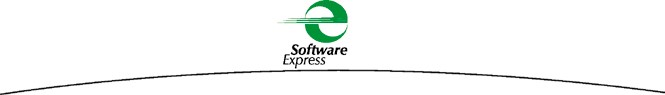
\includegraphics[width=1\textwidth,height=1.2\textheight,keepaspectratio]{fundoSE}
%\FloatBarrier
\end{figure}

\newcolumntype{C}[1]{>{\centering\let\newline\\\arraybackslash\hspace{0pt}}m{#1}}

\begin{center}
\setstretch{2}
    \begin{tabular}{|C{16.60cm}|}
        \hline
        RELATÓRIO DE DUPLA VERIFICAÇÃO – MÓDULOS SiTef \\
        D E C L A R A Ç Ã O \\
        \hline
    \end{tabular}
\end{center}

\medskip
\begin{table}[htbp]
\setstretch{1.9}
    \begin{tabular}{|lp{13.4cm}|}
    \cline{1-2}
    Data Verificação: & 
    VXX/XX/XXXXX 
    \\
    Nome do Módulo: & 
    XXXXXXXX.exe 
    \\
    Versão: & 
    VX.X.XX.XX 
    \\
    Projetista: & 
    PXXXXXXXXXX
    \\
    Conferente: & 
    CXXXXXXXXXX
    \\
    \cline{1-2}
    \end{tabular}%
\end{table}%
\medskip
    \label{tab:daypack}
\setstretch{1.5}
    \begin{tabularx}{\linewidth}{|l|l|p{11.3cm}|}
    \cline{1-3}
    \multicolumn{3}{|c|}{
    \large Alterações (em relação à versão anterior)} \\
    \cline{1-3}
    \multicolumn{1}{|c|}{
    \large Data} & 
    \multicolumn{1}{c|}{
    \large Versão Interna} & 
    \multicolumn{1}{c|}{
    \large Descrição} \\
    \cline{1-3}
    CXX/XX/XXXX 
    &
    CX.X.XX.XX 
    &
    -XXXXXXXXXX
    \\
    \cline{1-3}
    %\bottomrule
\end{tabularx}

\begin{flushleft}
 Certifico que o módulo supramencionado foi conferido segundo as Regras e Padrões internos da Software Express para Desenvolvimento de Software e o mesmo encontra-se aderente aos padrões existentes na data.
\medskip

\end{flushleft}


\begin{flushright}
\_\_\_\_\_\_\_\_\_\_\_\_\_\_\_\_\_\_\_\_\_\_\_\_\_\_\_\_\_\_\_\_\_\_

Assinatura do responsável pela implementação do módulo
\end{flushright}

\begin{flushright}

\end{flushright}

\begin{flushright}
\_\_\_\_\_\_\_\_\_\_\_\_\_\_\_\_\_\_\_\_\_\_\_\_\_\_\_\_\_\_\_\_\_\_

Assinatura do responsável pela conferência
\end{flushright}
\stopunderscoreletter

\end{document} 